% Scalar instruction entry source: tools/generate_scalar_instruction_catalog.py.
\subsection{\texttt{REMW}}
\label{sec:scalar-remw}
\index{REMW@\texttt{REMW}}
\begin{sloppypar}\noindent\textbf{Purpose.} Word (32-bit) integer remainder (signed).\end{sloppypar}\smallskip
\noindent\textbf{Syntax.}\par
\begin{lstlisting}[style=ptoscalarcode]
remw SrcL, SrcR, ->RegDst
\end{lstlisting}
\noindent\textbf{Encoding.}\par
\noindent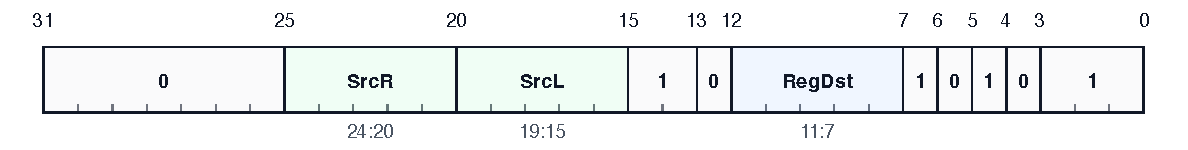
\includegraphics[width=\textwidth]{figs/encoding/scalar_instruction_entries/enc_remw.pdf}\par\smallskip
\begin{description}[leftmargin=0.18\linewidth,style=nextline]
\item[Format] \texttt{L32} \texttt{32-bit} scalar word.
\item[Pattern] \texttt{0000000..........110.....1010111}.
\end{description}
\noindent\textbf{Classification.}\par
\begin{description}[leftmargin=0.18\linewidth,style=nextline]
\item[Category] Integer ALU and Bit-Manipulation.
\item[Family] Multi-Cycle ALU.
\item[Execution class] \texttt{ALU}; uop\_kind=ALU, alu\_kind=ALU\_MULTI\_CYCLE.
\end{description}
\noindent\textbf{Operand fields.}\par
\begin{description}[leftmargin=0.18\linewidth,style=nextline]
\item[\texttt{RegDst}] Bits \texttt{11:7 (5b)}. 5-bit scalar destination register written by this instruction; X0 is hardwired to zero, so writes to X0 are ignored.
\item[\texttt{SrcL}] Bits \texttt{19:15 (5b)}. 5-bit scalar source register used as the left input operand.
\item[\texttt{SrcR}] Bits \texttt{24:20 (5b)}. 5-bit scalar source register used as the right input operand before any encoded modifier or shift is applied.
\end{description}
\noindent\textbf{Operation.}\par
\begin{lstlisting}[style=ptoscalarcode]
a = Read(SrcL)[31:0]
b = Read(SrcR)[31:0]
if (b == 0):
  result = a
else:
  // signed overflow: MIN_INT / -1
  q = TruncTowardZeroDiv(a, b)
  result = a - q*b
  result = SignExtend32(result)
Write(RegDst, result)
\end{lstlisting}
\Needspace{0.08\textheight}
